\chapter{Invasive Computing}\label{chapter:invasive computing}
\section{Job Classification}
\section{Resource Aware Programming}

\section{Traditional Resource Management}
The role of a resource manager is to acts like a \textit{glue} for a parallel computer to execute parallel jobs. It should make a parallel computer as easy to use as almost a PC. MPI would typically be used to manage communications within the parallel program. A resource manager allocates resources within a cluster, launches and otherwise manages jobs. Some of the examples of widely used open source as well as commercial resource managers are \textbf{SLURM, TORQUE, OMEGA, IBM Platform LSF} etc. Together with a scheduler it is termed as a \textbf{\textit{Batch System}}. The Batch System serves as a middleware for managing supercomputing resources. The combination of \textit{Scheduler}$+$\textit{Resource Manager} makes it possible to run parallel jobs.\par
\noindent
\\
The role of a job scheduler is to manage queue(s) of work when there is more work than resources. It supports complex scheduling algorithms which are optimized for network topology, energy efficiency, fair share scheduling, advanced reservations, preemption, gang scheduling(time-slicing jobs) etc. It also supports resource limits(by queue, user, group, etc.). Many batch systems provide both resource management and job scheduling within a single product (e.g. LSF) while others use distinct products(e.g. Torque resource manager and Moab job scheduler). Some other examples of Job scheduling systems are \textbf{LoadLeveler, OAR, Maui, SLURM} etc.\par
\noindent
\\
The prime focus of this work will be on \textbf{SLURM(Simple Linux Utility For Resource Management)} which will be the choice of batch system upon which the support for Invasive Computing will be demonstrated. SLURM is a sophisticated open source batch system with about 500,000 lines of C code whose development started in the year 2002 at Lawrence Livermore National Laboratory as a simple resource manager for Linux Clusters and a few years ago spawned into an independent firm under the name SchedMD. SLURM has since its inception also evolved into a very capable job scheduler through the use of optional plugins. It is used on many of the world's largest supercomputers and is used by a large fraction of the world's TOP500 Supercomputer list. It supports many UNIX falvors like AIX, Linux, Solaris and is also fault tolerant, highly scalable, and portable.\par
\noindent
\\
\textbf{Plugins} are dynamically linked objects loaded at run time based upon configuration file and/or user options. \ref{fig:6} shows where these plugins fit inside SLURM. Approximately $80$ plugins of different varities are currently available. Some of them are listed below:\\
\begin{itemize}
\item \textbf{\textit{Accounting storage:}} MySQL, PostgreSQL, textfile.
\item \textbf{\textit{Network Topology:}} 3D-Torus, tree.
\item \textbf{\textit{MPI:}} OpenMPI, MPICH1, MVAPICH, MPICH2, etc.
\end{itemize}
PLugins are typically loaded when the daemon or command starts and persist indefinitely. They provide a level of indirection to a configurable underlying function.
\begin{figure}[h]
\centering
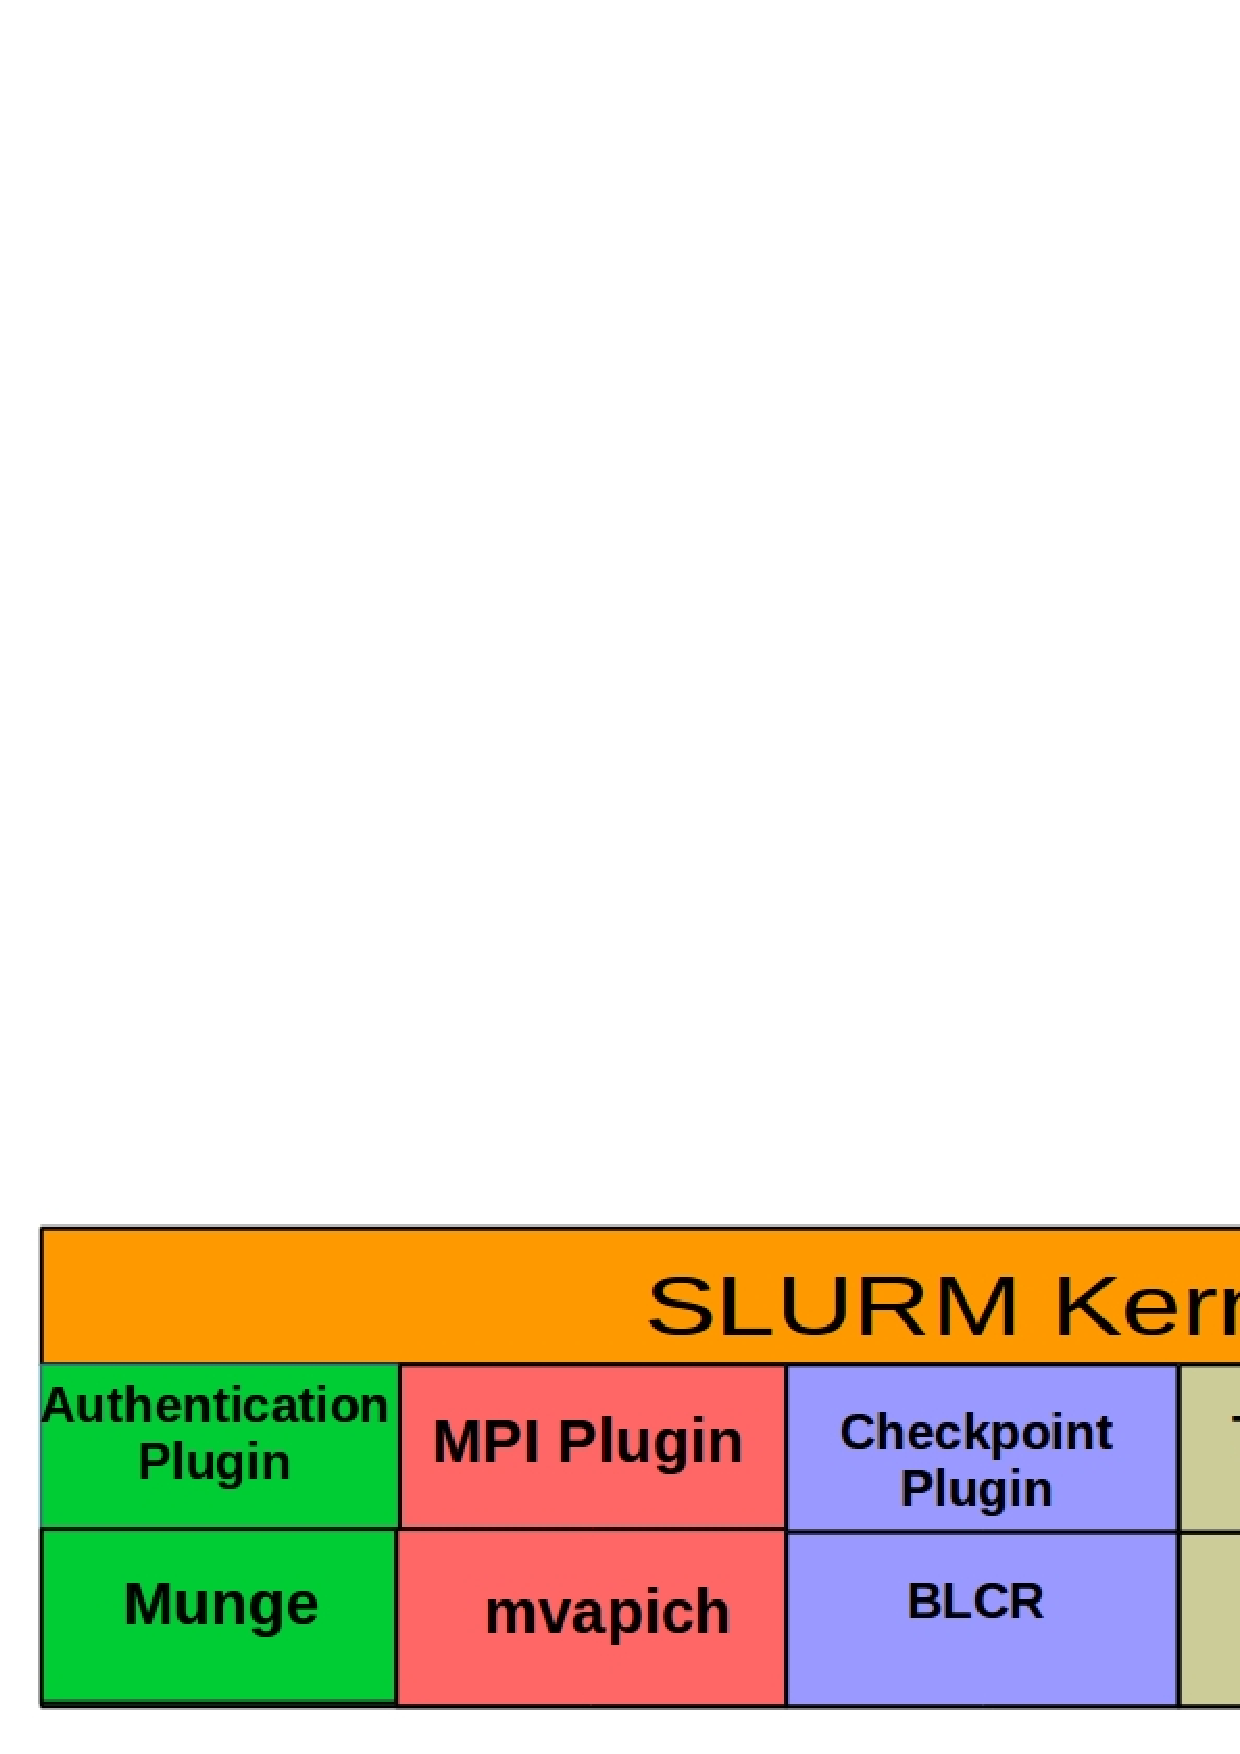
\includegraphics[width=1.0\textwidth]{./figures/plugin.pdf}
\vspace{-0.15in}
\caption{SLURM with optional Plugins}
\label{fig:6}
\end{figure}


\section{Support for Invasive Computing}
\subsection{Invasive MPI}

\subsection{Resource Management Extensions}
Existing batch systems usually only support static allocation of resources to applications before job start. Hence we need some kind of an Invasive Resource Management to be integrated into these existing batch systems so that we can support malleable jobs allowing us to change the allocated resources dynamically at runtime. In order to achieve this we will follow the below approach:
\begin{itemize}
\item \textbf{\textit{Invasive Resource Manager (alias iHypervisor):}} An independent component which will talk to the current batch systems via a communication mechanism(protocol) to obtain invasive job(s) submitted specifically to the invasic partition that can support invasive computing. The iHypervisor will then take these jobs and perform some kind of runtime scheduling for pinning these jobs to the resources in the partition and makes these decisions in order to optimize certain local metrics such as resource utilization, power stability, energy efficiency etc. The scheduling here is done at the granularity of cores and sockets. iHypervisor is the one that has the complete information of the resources in the invasic partition and also manages them. This component in an independent entity with the purpose of inter-operating with existing batch systems rather than replacing them with an entirely new one. It may be possible that in the future this component will not be a separate entitiy but will be built into the batch system itself.
\item \textbf{\textit{Invasive Job Scheduler (alias iScheduler):}} This component will be a new extension built into the existing batch systems for performing job scheduling. The scheduling decisions are communicated via the protocol used to speak to iHypervisor and these decisions are basically job(s) selected via a scheduling algorithm to be submitted to the iHypervisor for execution. The scheduling decisions will be made on the basis of available resources in the partition and it is the iHypervisor that communicates this to iScheduler in the form of resource offers (Real/Virtual). It can be a virtual resource offer because the iHypervisor can hide the real resources and present a rather fake view of them to iScheduler in the hope of getting a mapping of jobs to offer that is more suitable to satisfy its local metrics. Similar to iHypervisor, the iScheduler makes its decisions to optimize for certain local metrics such as high job throughput, reduced job waiting times, deadlines, priorities etc. This highlights the mismatching policies/metrics for which both the iHypervisor and iScheduler make their decisions on and hence both will be involved in some kind of a negotiation via the protocol to reach a common agreement.
\item \textbf{\textit{Negotiation Protocol:}} This protocol forms the core of the interaction between the iScheduler and iHypervisor. It allows for iHypervisor to make one or a set of resource offers to iScheduler which then needs to select jobs from its job queue to be mapped to these resource offers and finally sent back to the iHypervisor. The iHypervisor will then decide whether to accept/reject this mapping to satisfy its local metrics. If it accepts it will launch them based on some run time scheduling and if it rejects then it informs this to iScheduler in addition to sending it a new resource offer. The iScheduler can also reject the resource offers in which case it will be sent a new one. On accepting an offer, the iScheduler then repeats its tasks to send back a mapping to iHypervisor and this interaction continues until both reach a common agreement. If the number of such attempts reach a threshold then iScheduler will just accept whatever offer it receives and iHypervisor will also accept whatever Map:Jobs$\rightarrow$Offers it receives closing this transaction of negotiating. After this a new transaction will start.
\item \textbf{\textit{SLURM:}} SLURM is our choice of an existing batch system upon which this new implementation will be demonstrated as a proof of concept to support the new paradigm of resource-aware programming in the domain of invasive computing. In the near future, This can motivate further such supporting infrastructures with other batch systems using such Invasive Resource Management and Scheduling components.
\end{itemize}
\noindent
This project implements a testing prototype for demonstrating how such an approach to support invasive computing with the above entities may work. It will involve implementing the communication infrastructure using SLURM API due to which iHypervisor and iScheduler will interact with each other using protocol messages filled with dummy values. It will also involve implementing the iScheduler as a new plugin(multithreaded) for SLURM and iHypervisor as a fake multithreaded Invasive Resource Manager daemon with bare minimum functionalities that in the near future will be an enhanced version of the daemon slurmd(built on top of it) found in SLURM. For the purposes of testing this prototype, the different scenarios that can be observed most of the time with the kind of negotiation protocol described earlier would be verified.
